% \chapter{卷积神经网络的基础知识}
% \section{卷积神经网络的网络结构}
% 卷积神经网络作为深度学习的一个分支,在网络结构上同样含有深度学习的“深度”性。网络拓扑结构是一个多层的神经网络\overcite{ref8},网络的每一层由多个独立的神经元组成的二维平面组成。网络一般分为输入层、卷积层、池化层、全连接层、输出层等。
% \subsection{输入层}
% 因为卷积神经网络可以直接的接受二维的视觉模式\overcite{ref9},所以我们可以直接把简单预处理后的二维图像输入到输入层中。
% \subsection{输出}
% ……
% \section{卷积神经网络的学习规律}
% ……
% \subsection{前向传播}
% 如果用$l$来表示当前的网络层,那么当前网络层的输出如\autoref{eq:fp}所示:
% \begin{equation}
%     \label{eq:fp}
%     {x^l} = f({u^l}),\text{其中}{u^l} = {W^l}{x^{l - 1}} + {b^l}
% \end{equation}
% 其中$f(\cdot)$为网络的输出激活函数。在本文实验中,网络的输出激活函数选用sigmoid函数,因此网络的输出均值一般来说趋于0。
% \subsection{反向传播}
% ……
% \subsection{学习特征图的组合}
% ……
% \section{本章小结}
% ……

\chapter{状态空间模型} 
\section{状态空间模型}
用数学术语来说,状态空间模型 (SSM) 中的最优滤波和平滑可以表述为统计反演问题。我们的目标是从一组噪声观测值 \(\{\mathbf{y}_1, \mathbf{y}_2, \dots\}\) 中估计一个未知的向量值时间序列 \(\{\mathbf{x}_0, \mathbf{x}_1, \mathbf{x}_2, \dots\}\)。为了方便记述,我们定义 \(\textbf{x}_{0:T} = \{ \textbf{x}_0, \textbf{x}_1, \dots, \textbf{x}_T \}\) 和 \(\textbf{y}_{1:T} = \{ \textbf{y}_1, \textbf{y}_2, \dots, \textbf{y}_T \}\)。

贝叶斯滤波解决了一般概率状态空间模型中的状态估计问题,这些模型的特征如下:
\begin{align*}
\mathbf{x}_k &\sim p(\mathbf{x}_k \mid \mathbf{x}_{k-1}), \\
\mathbf{y}_k &\sim p(\mathbf{y}_k \mid \mathbf{x}_k),
\end{align*}
其中 \(k = 1, 2, \dots\),其中:
\begin{itemize}
\item \(\mathbf{x}_k \in \R^n\) 表示系统在时间步 \(k\) 的状态,
\item \(\mathbf{y}_k \in \R^m\) 表示时间步 \(k\) 的测量值\(k\),
\item \(p(\mathbf{x}_k \mid \mathbf{x}_{k-1})\) 是动态模型,描述系统的随机演化。
\item \(p(\mathbf{y}_k \mid \mathbf{x}_k)\) 是测量模型,表示给定状态下观测值的似然值。
\end{itemize}

\subsection{用于最优过滤的贝叶斯推断}
在 SSM 的背景下,主要关注的是估计给定相应观测值的所有状态的联合后验分布。该分布由以下公式给出:
\begin{align*}
p(\mathbf{x}_{0:T} \mid \mathbf{y}_{1:T}) = \frac{p(\mathbf{y}_{1:T} \mid \mathbf{x}_{0:T}) p(\mathbf{x}_{0:T})}{p(\mathbf{y}_{1:T})},
\end{align*}
其中:
\begin{itemize}
\item \(p(\mathbf{x}_{0:T})\) 是状态的先验分布,
\item \(p(\mathbf{y}_{1:T} \mid \mathbf{x}_{0:T})\) 是给定状态下观测值的似然值,
\item \(p(\mathbf{y}_{1:T})\) 是归一化常数,确保后验分布积分为 1。
\end{itemize}

\subsection{关键边际分布}
在实践中,我们通常对由联合后验推导的特定边际分布感兴趣。这些分布包括:
\begin{itemize}
\item \textit{滤波分布},它根据所有过去和当前的观测值估计当前状态:
\begin{align*}
\left\{ p(\mathbf{x}_k \mid \mathbf{y}_{1:k}) \mid k = 1, \dots, T \right\}。
\end{align*}
\item \textit{预测分布},根据当前观测值预测未来状态:
\begin{align*}
\left\{ p(\mathbf{x}_{k+n} \mid \mathbf{y}_{1:k}) \mid k = 1, \dots, T, \, n = 1, 2, \dots \right\}。
\end{align*}
\item \textit{平滑分布},利用所有可用观测值改进过去的状态估计:
\begin{align*}
\left\{ p(\mathbf{x}_k \mid \mathbf{y}_{1:T}) \mid k = 1, \dots, T \right\}。
\end{align*}
\end{itemize}
这些分布构成了贝叶斯滤波和平滑的基础,从而能够在 SSM 中实现准确的状态估计和预测。

\section{线性高斯状态空间模型}
卡尔曼滤波器是贝叶斯滤波器的一个特例,其中动态模型和测量模型均为线性高斯模型。该模型由以下方程定义:
\begin{align*}
\mathbf{x}_k &= \mathbf{A}_{k-1} \mathbf{x}_{k-1} + \mathbf{q}_{k-1}, \\
\mathbf{y}_k &= \mathbf{H}_k \mathbf{x}_k + \mathbf{r}_k,
\end{align*}
其中:
\begin{itemize}
\item \(\mathbf{q}_{k-1} \sim \mathcal{N}(\mathbf{0}, \mathbf{Q}_{k-1})\) 是过程噪声,假设为具有零均值和协方差的高斯分布\(\mathbf{Q}_{k-1}\),
\item \(\mathbf{r}_k \sim \mathcal{N}(\mathbf{0}, \mathbf{R}_k)\) 为测量噪声,假设为均值为零、协方差为 \(\mathbf{R}_k\) 的高斯分布。
\item \(\mathbf{x}_0 \sim \mathcal{N}(\mathbf{m}_0, \mathbf{P}_0)\) 为初始状态,假设为均值为 \(\mathbf{m}_0\)、协方差为 \(\mathbf{P}_0\) 的高斯分布。
\item \(\mathbf{A}_{k-1}\) 为状态转移矩阵。
\item \(\mathbf{H}_k\) 是观测矩阵。
\end{itemize}

或者,该模型可以用概率术语表示为:
\begin{align*}
 p(\mathbf{x}_k \mid \mathbf{x}_{k-1}) &\sim \mathcal{N}(\mathbf{x}_k \mid \mathbf{A}_{k-1} \mathbf{x}_{k-1}, \mathbf{Q}_{k-1}), \\
 p(\mathbf{y}_k \mid \mathbf{x}_k) &\sim \mathcal{N}(\mathbf{y}_k \mid \mathbf{H}_k \mathbf{x}_k, \mathbf{R}_k)。
\end{align*}

\begin{figure}[tb]
\centering
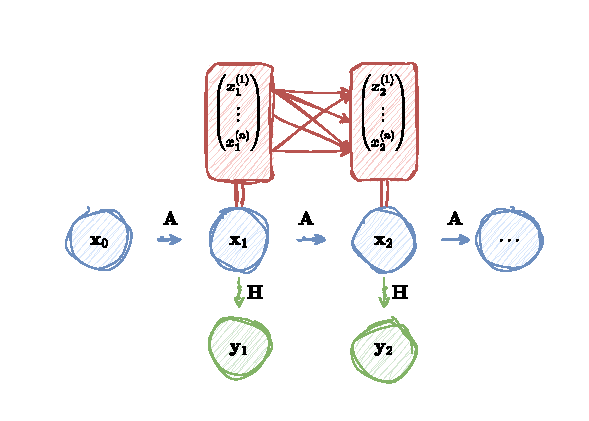
\includegraphics[width=0.75\linewidth]{fig/Markov Chian.pdf}
\caption{\textit{线性高斯状态空间模型}的流程。\textcolor{blue}{蓝色块}表示\textit{转换过程},\textcolor{red}{红色块}说明\textit{马尔可夫链属性}的细节,\textcolor{green}{绿色块}表示\textit{观察过程}。}
\label{fig: LGSSM 流程图}
\end{figure}

图~\ref{fig: LGSSM 流程图} 展示了线性高斯状态空间模型 (LGSSM) 的流程。蓝色块表示状态转换过程,描述系统随时间的变化。红色块突出了模型的马尔可夫属性,强调当前状态仅依赖于先前状态。绿色块表示观察过程,将状态映射到观察到的测量值。

\subsection{卡尔曼滤波器}
卡尔曼滤波器为线性高斯状态空间模型 (LGSSM) 中的状态估计问题提供了递归解决方案。卡尔曼滤波器涉及的关键分布是:
\begin{align}
 p(\mathbf{x}_k \mid \mathbf{y}_{1:k-1}) &\sim \mathcal{N}(\mathbf{x}_k \mid \mathbf{m}_k^-, \mathbf{P}_k^-), \\
 p(\mathbf{x}_k \mid \mathbf{y}_{1:k}) &\sim \mathcal{N}(\mathbf{x}_k \mid \mathbf{m}_k, \mathbf{P}_k), \\
 p(\mathbf{y}_k \mid \mathbf{y}_{1:k-1}) &\sim \mathcal{N}(\mathbf{y}_k \mid \mathbf{H}_k \mathbf{m}_k^-, \mathbf{S}_k)。\label{eq: single likelihood}
\end{align}

\subsubsection*{预测步骤}
预测步骤使用动态模型将状态估计及其不确定性从上一个时间步传播到当前时间步。预测步骤的公式如下:
\begin{align*}
\mathbf{m}_k^- &= \mathbf{A}_{k-1} \mathbf{m}_{k-1}, \\
\mathbf{P}_k^- &= \mathbf{A}_{k-1} \mathbf{P}_{k-1} \mathbf{A}_{k-1}^\mathsf{T} + \mathbf{Q}_{k-1}.
\end{align*}
其中,\(\mathbf{m}_k^-\) 和 \(\mathbf{P}_k^-\) 分别表示预测状态均值和协方差。

\subsubsection*{更新步骤}
更新步骤结合新的观测值 \(\mathbf{y}_k\) 来优化预测状态估计。更新步骤的方程为:
\begin{align}
 \mathbf{v}_k &= \mathbf{y}_k - \mathbf{H}_k \mathbf{m}_k^-, \label{eq: kalman filter vk} \\
 \mathbf{S}_k &= \mathbf{H}_k \mathbf{P}_k^- \mathbf{H}_k^\mathsf{T} + \mathbf{R}_k, \label{eq: kalman filter Sk} \\
 \mathbf{K}_k &= \mathbf{P}_k^- \mathbf{H}_k^\mathsf{T} \mathbf{S}_k^{-1}, \\
\mathbf{m}_k &= \mathbf{m}_k^- + \mathbf{K}_k \mathbf{v}_k, \\
\mathbf{P}_k &= \mathbf{P}_k^- - \mathbf{K}_k \mathbf{S}_k \mathbf{K}_k^\mathsf{T}.
\end{align}
其中,\(\mathbf{v}_k\) 为残差,\(\mathbf{S}_k\) 为残差协方差,\(\mathbf{K}_k\) 为卡尔曼增益,\(\mathbf{m}_k\) 和 \(\mathbf{P}_k\) 分别为更新后的状态均值和协方差。

\subsection{卡尔曼平滑器}
卡尔曼平滑器扩展了卡尔曼滤波器,它使用所有可用的观测值 \(\mathbf{y}_{1:T}\) 来估计每个时间步 \(k\) 的状态。具体来说,它计算平滑分布:
\begin{align*}
p(\mathbf{x}_k \mid \mathbf{y}_{1:T}) \sim \mathcal{N}(\mathbf{x}_k \mid \mathbf{m}_k^s, \mathbf{P}_k^s),
\end{align*}
其中 \(\mathbf{m}_k^s\) 和 \(\mathbf{P}_k^s\) 分别是平滑后的状态均值和协方差。

\subsubsection*{向后递归方程}
卡尔曼平滑器通过向后递归进行运算,从最终时间步长 \(T\) 开始,向后递归到初始时间步长 \(0\)。

\section{状态空间模型中的参数估计}
在贝叶斯框架中,缺失参数 \(\boldsymbol{\theta} \in \R^d\) 被视为具有先验分布 \(p(\boldsymbol{\theta})\) 的随机变量。包含这些缺失参数的状态空间模型 (SSM) 定义为:
\begin{align*}
\boldsymbol{\theta} &\sim p(\boldsymbol{\theta}), \\
\mathbf{x}_0 &\sim p(\mathbf{x}_0 \mid \boldsymbol{\theta}), \\
\mathbf{x}_k &\sim p(\mathbf{x}_k \mid \mathbf{x}_{k-1}, \boldsymbol{\theta}), \\
\mathbf{y}_k &\sim p(\mathbf{y}_k \mid \mathbf{x}_k, \boldsymbol{\theta})。
\end{align*}

参数估计的基本方法基于贝叶斯规则,该规则将给定观测值的状态和参数的联合后验分布表示为:
\begin{align*}
p(\mathbf{x}_{0:T}, \boldsymbol{\theta} \mid \mathbf{y}_{1:T}) = \frac{p(\mathbf{y}_{1:T} \mid \mathbf{x}_{0:T}, \boldsymbol{\theta}) \, p(\mathbf{x}_{0:T} \mid \boldsymbol{\theta}) \, p(\boldsymbol{\theta})}{p(\mathbf{y}_{1:T})},
\end{align*}
其中:
\begin{itemize}
\item \(p(\mathbf{x}_{0:T} \mid \boldsymbol{\theta}) = p(\mathbf{x}_0 \mid \boldsymbol{\theta}) \prod_{k=1}^{T} p(\mathbf{x}_k \mid \mathbf{x}_{k-1}, \boldsymbol{\theta})\) 是状态的先验分布,
\item \(p(\mathbf{y}_{1:T} \mid \mathbf{x}_{0:T}, \boldsymbol{\theta}) = \prod_{k=1}^{T} p(\mathbf{y}_k \mid \mathbf{x}_k, \boldsymbol{\theta})\) 是观测值。
\end{itemize}

参数估计的核心目标是找到最大化边缘后验分布的后验模态 \(\boldsymbol{\theta}\):
\begin{align*}
\boldsymbol{\theta} = \arg \max_{\boldsymbol{\theta}} p(\boldsymbol{\theta} \mid \mathbf{y}_{1:T})。
\end{align*}
这本质上是一个优化问题。然而,在解决这个问题之前,我们必须先解决计算 \(p(\boldsymbol{\theta} \mid \mathbf{y}_{1:T})\) 的难题。

为了集中计算 \(p(\boldsymbol{\theta} \mid \mathbf{y}_{1:T})\),即 \(\boldsymbol{\theta}\) 的边缘后验分布,直接求解方法涉及对状态进行边缘化:
\begin{align*}
p(\boldsymbol{\theta} \mid \mathbf{y}_{1:T}) = \int p(\mathbf{x}_{0:T}, \boldsymbol{\theta} \mid \mathbf{y}_{1:T}) \, \mathrm{d} \mathbf{x}_{0:T}.
\end{align*}

遗憾的是,计算这个高维积分极具挑战性,而且随着测量值的增多,计算难度也会越来越大。为了解决这个问题,我们提出了一些参数估计方法,该方法可以近似边缘后验分布 \(p(\boldsymbol{\theta} \mid \mathbf{y}_{1:T})\),而无需明确构建联合后验分布 \(p(\mathbf{x}_{0:T}, \boldsymbol{\theta} \mid \mathbf{y}_{1:T})\)。具体来说,我们关注:
\begin{align*}
p(\boldsymbol{\theta} \mid \mathbf{y}_{1:T}) \propto p(\mathbf{y}_{1:T} \mid \boldsymbol{\theta}) p(\boldsymbol{\theta})。
\end{align*}

因此,问题简化为计算 \textit{似然值} \(p(\mathbf{y}_{1:T} \mid \boldsymbol{\theta})\)。 (先验项 \(p(\boldsymbol{\theta})\) 是根据先验知识选择的,而归一化常数 \(p(\mathbf{y}_{1:T})\) 则被贝叶斯理论所避免。)

估计这种似然值的关键在于状态空间模型中的递归计算,也称为因式分解或预测误差分解:
\begin{align*}
p(\mathbf{y}_{1:T} \mid \boldsymbol{\theta}) = \prod^T_{k=1} p(\mathbf{y}_k \mid \mathbf{y}_{1:k-1}, \boldsymbol{\theta}),
\end{align*}
其中:
\begin{itemize}
\item \(p(\mathbf{y}_1 \mid \mathbf{y}_{1:0}, \boldsymbol{\theta}) \triangleq p(\mathbf{y}_1 \mid \boldsymbol{\theta})\)。
\end{itemize}

处理 \(p(\mathbf{y}_k \mid \mathbf{y}_{1:k-1}, \boldsymbol{\theta})\) 的核心思想是:
\begin{align*}
 p(\mathbf{y}_k \mid \mathbf{y}_{1:k-1}, \boldsymbol{\theta}) &= \int p(\mathbf{y}_k \mid \mathbf{x}_k, \boldsymbol{\theta}) \, p(\mathbf{x}_k \mid \mathbf{y}_{1:k-1}, \boldsymbol{\theta}) \, \mathrm{d} \mathbf{x}_k, \\
 p(\mathbf{x}_k \mid \mathbf{y}_{1:k}, \boldsymbol{\theta}) &= \frac{p(\mathbf{y}_k \mid \mathbf{x}_k, \boldsymbol{\theta}) \, p(\mathbf{x}_k \mid \mathbf{y}_{1:k-1}, \boldsymbol{\theta})}{p(\mathbf{y}_k \mid \mathbf{y}_{1:k-1}, \boldsymbol{\theta})},
\end{align*}
其中:
\begin{itemize}
 \item \(p(\mathbf{y}_k \mid \mathbf{x}_k, \boldsymbol{\theta})\) 是 \textit{测量模型},
 \item \(p(\mathbf{x}_k \mid \mathbf{y}_{1:k-1}, \boldsymbol{\theta})\) 是状态 \(\mathbf{x}_k\) 的 \textit{预测分布},由以下公式给出:
\begin{align*}
p(\mathbf{x}_k \mid \mathbf{y}_{1:k-1}, \boldsymbol{\theta}) = \int p(\mathbf{x}_k \mid \mathbf{x}_{k-1}, \boldsymbol{\theta}) p(\mathbf{x}_{k-1} \mid \mathbf{y}_{1:k-1}, \boldsymbol{\theta}) \, \mathrm{d} \mathbf{x}_{k-1}。
\end{align*}
\item \(p(\mathbf{x}_k \mid \mathbf{y}_{1:k}, \boldsymbol{\theta})\) 是 \textit{贝叶斯滤波器}。
\end{itemize}

注意,上述方程求解了状态空间模型中的似然函数。对于线性高斯状态空间模型的特殊情况,通过利用卡尔曼滤波器的结果,似然的计算得到了显著的简化。

\subsection{具有缺失参数的线性高斯状态空间模型}

具有缺失参数 \(\boldsymbol{\theta}\) 的线性高斯状态空间模型(LGSSM)定义为:
\begin{align*}
    \mathbf{x}_k &= \mathbf{A}(\boldsymbol{\theta}) \, \mathbf{x}_{k-1} + \mathbf{q}_{k-1}, \\
    \mathbf{y}_k &= \mathbf{H}(\boldsymbol{\theta}) \, \mathbf{x}_k + \mathbf{r}_k,
\end{align*}
其中:
\begin{itemize}
    \item \(\mathbf{q}_{k-1} \sim \mathcal{N}(\mathbf{0}, \mathbf{Q}(\boldsymbol{\theta}))\) 和 \(\mathbf{r}_{k} \sim \mathcal{N}(\mathbf{0}, \mathbf{R}(\boldsymbol{\theta}))\) 分别是过程噪声和测量噪声,
    \item \(\mathbf{x}_0 \sim \mathcal{N}(\mathbf{m}_0(\boldsymbol{\theta}), \mathbf{P}_0(\boldsymbol{\theta}))\) 是初始状态分布,
    \item 假设模型参数 \(\boldsymbol{\theta}\) 是时间不变的。
\end{itemize}

在接下来的章节中,我们将介绍应对 LGSSM 中计算和优化挑战的实用方法,具体包括梯度下降算法和期望最大化(EM)算法。

\subsection{梯度下降算法}

我们从方程~\eqref{eq: single likelihood} 中知道,\(p(\mathbf{y}_k \mid \mathbf{y}_{1:k-1}, \boldsymbol{\theta})\) 的分布是高斯分布:
\[
p(\mathbf{y}_k \mid \mathbf{y}_{1:k-1}, \boldsymbol{\theta}) \sim \mathcal{N}(\mathbf{H}_k(\boldsymbol{\theta}) \, \mathbf{m}_k^-(\boldsymbol{\theta}), \mathbf{S}_k(\boldsymbol{\theta})).
\]
因此,对数似然 \(\log p(\mathbf{y}_{1:T} \mid \boldsymbol{\theta})\) 可以表示为从正态分布推导出的递归求和项:
\begin{align*}
    \log p(\mathbf{y}_{1:T} \mid \boldsymbol{\theta}) = \sum^T_{k=1} \left( \frac{1}{2} \log | 2 \pi \, \mathbf{S}_k(\boldsymbol{\theta}) | + \frac{1}{2} \mathbf{v}_k^{\mathsf{T}}(\boldsymbol{\theta}) \, \mathbf{S}_k^{-1}(\boldsymbol{\theta}) \, \mathbf{v}_k (\boldsymbol{\theta}) \right),
\end{align*}
其中:
\begin{itemize}
    \item \(\mathbf{v}_k (\boldsymbol{\theta})\) 和 \(\mathbf{S}_k(\boldsymbol{\theta})\) 分别是残差值和残差协方差,定义见卡尔曼滤波器中的方程~\eqref{eq: kalman filter vk} 和方程~\eqref{eq: kalman filter Sk},
    \item \(m\) 是观测空间的维度,满足 \(\mathbf{y} \in \R^m\)。
\end{itemize}

令 \(\ell(\boldsymbol{\theta}) \triangleq \log p(\mathbf{y}_{1:T} \mid \boldsymbol{\theta})\)。为了最大化对数似然,我们使用梯度下降算法,该算法通过以下方式迭代更新参数估计 \(\boldsymbol{\theta}\):
\begin{align*}
    \boldsymbol{\theta}^{(i+1)} = \boldsymbol{\theta}^{(i)} - \eta \, \nabla_{\boldsymbol{\theta}} \ell(\boldsymbol{\theta}^{(i)}),
\end{align*}
其中:
\begin{itemize}
    \item \(\eta > 0\) 是学习率,控制更新的步长,
    \item \(\nabla_{\boldsymbol{\theta}} \ell(\boldsymbol{\theta})\) 是对数似然关于 \(\boldsymbol{\theta}\) 的梯度,
    \item \(\boldsymbol{\theta}^{(i)}\) 是第 \(i\) 次迭代中的参数估计。
\end{itemize}

梯度 \(\nabla_{\boldsymbol{\theta}} \ell(\boldsymbol{\theta})\) 可以使用链式法则计算,利用卡尔曼滤波器的递归性质。具体而言,\(\mathbf{v}_k(\boldsymbol{\theta})\) 和 \(\mathbf{S}_k(\boldsymbol{\theta})\) 的梯度项由卡尔曼滤波器方程推导得到,整体梯度通过求和所有时间步 \(k = 1, \dots, T\) 的贡献得到。

\subsection{EM 算法}
\paragraph*{状态空间模型的 EM 算法}
令 \(q(\mathbf{x}_{0:T})\) 为状态 \(\mathbf{x}_{0:T}\) 上的任意概率密度函数。对于对数似然 \(\log p(\mathbf{y}_{1:T} \mid \boldsymbol{\theta})\),总是存在一个下界,如下所示:
\begin{align}
    \log p(\mathbf{y}_{1:T} \mid \boldsymbol{\theta}) \ge F(q(\mathbf{x}_{0:T}), \boldsymbol{\theta}), \label{eq: ineq for EM}
\end{align}
其中二元函数 \(F(\cdot)\) 定义为:
\begin{align*}
    F(q(\mathbf{x}_{0:T}), \boldsymbol{\theta}) = \int q(\mathbf{x}_{0:T}, \boldsymbol{\theta}) \, \log \frac{p(\mathbf{x}_{0:T}, \mathbf{y}_{1:T} \mid \boldsymbol{\theta})}{q(\mathbf{x}_{0:T}, \boldsymbol{\theta})} \, \mathrm{d} \mathbf{x}_{0:T}.
\end{align*}

这自然引出了算法~\ref{alg: abstract EM},用于求解这个优化问题。

\begin{algorithm}[tb]
    \caption{简略 EM 算法}
    \label{alg: abstract EM}
    \begin{algorithmic}[1]
        \ENSURE{\(\boldsymbol{\theta}^{(N)}\)}
        \STATE \(\boldsymbol{\theta}^{(0)} \gets \text{随机值}\)
        \FOR{\(n = 0, 1, \dots, N-1\)}
            \STATE E 步骤:\(q^{(n+1)}(\cdot) \gets \arg \max_{q(\cdot)} F(q(\cdot), \boldsymbol{\theta}^{(n)})\)。
            \STATE M 步骤:\(\boldsymbol{\theta}^{(n+1)} \gets \arg \max_{\boldsymbol{\theta}} F(q^{(n+1)}(\cdot), \boldsymbol{\theta})\)。
        \ENDFOR
    \end{algorithmic}
\end{algorithm}

为了求解算法~\ref{alg: abstract EM} 中的 E 步骤,我们直接给出最优解:
\begin{align}
    q^{(n+1)}(\mathbf{x}_{0:T}) &= p(\mathbf{x}_{0:T} \mid \mathbf{y}_{1:T}, \boldsymbol{\theta}^{(n)}), \\
    F[q^{(n+1)}(\mathbf{x}_{0:T}), \boldsymbol{\theta}] &= \int p(\mathbf{x}_{0:T} \mid \mathbf{y}_{1:T}, \boldsymbol{\theta}^{(n)}) \log p(\mathbf{x}_{0:T}, \mathbf{y}_{1:T} \mid \boldsymbol{\theta}) \, \mathrm{d} \mathbf{x}_{0:T} \label{eq: full lower bound} \\
    &\quad - \int p(\mathbf{x}_{0:T} \mid \mathbf{y}_{1:T}, \boldsymbol{\theta}^{(n)}) \log p(\mathbf{x}_{0:T} \mid \mathbf{y}_{1:T}, \boldsymbol{\theta}^{(n)}) \, \mathrm{d} \mathbf{x}_{0{T}}. \nonumber
\end{align}

注意,方程~\eqref{eq: full lower bound} 中的第二项不依赖于 \(\boldsymbol{\theta}\)。因此,算法~\ref{alg: abstract EM} 中的 M 步骤优化可以简化,只考虑方程~\eqref{eq: full lower bound} 中的第一项作为对数似然的新下界,记作 \(\mathcal{Q}(\boldsymbol{\theta}, \boldsymbol{\theta}^{(n)})\):
\begin{align*}
    \mathcal{Q}(\boldsymbol{\theta}, \boldsymbol{\theta}^{(n)}) = \int p(\mathbf{x}_{0:T} \mid \mathbf{y}_{1:T}, \boldsymbol{\theta}^{(n)}) \log p(\mathbf{x}_{0:T}, \mathbf{y}_{1:T} \mid \boldsymbol{\theta}) \, \mathrm{d} \mathbf{x}_{0:T}.
\end{align*}

因此,我们得到了最终的迭代不等式,改编自方程~\eqref{eq: ineq for EM}:
\begin{align}
    \log p(\mathbf{y}_{1:T} \mid \boldsymbol{\theta}) \ge \mathcal{Q}(\boldsymbol{\theta}, \boldsymbol{\theta}^{(n)}). \label{eq: ineq for EM final}
\end{align}

这引出了简化版本的 EM 算法,用于估计状态空间模型的参数,如算法~\ref{alg: EM algorithm} 所示。

\begin{algorithm}[tb]
    \caption{状态空间模型的 EM 算法}
    \label{alg: EM algorithm}
    \begin{algorithmic}[1]
        \ENSURE{\(\boldsymbol{\theta}^{(N)}\)}
        \STATE \(\boldsymbol{\theta}^{(0)} \gets \text{随机值}\)
        \FOR{\(n = 0, 1, \dots, N-1\)}
            \STATE E 步骤:计算 \(\mathcal{Q}(\boldsymbol{\theta}, \boldsymbol{\theta}^{(n)})\)。
            \STATE M 步骤:\(\boldsymbol{\theta}^{(n+1)} \gets \arg \max_{\boldsymbol{\theta}} \mathcal{Q}(\boldsymbol{\theta}, \boldsymbol{\theta}^{(n)})\)。
        \ENDFOR
    \end{algorithmic}
\end{algorithm}

\paragraph*{线性高斯状态空间模型的 EM 算法}
在线性高斯状态空间模型(LGSSM)的假设下,\(\mathcal{Q}(\boldsymbol{\theta}, \boldsymbol{\theta}^{(n)})\) 的表达式为:
\begin{align}
    \mathcal{Q}(\boldsymbol{\theta}, \boldsymbol{\theta}^{(n)}) &= -\frac{1}{2} \log |2\pi \mathbf{P}_0(\boldsymbol{\theta})| - \frac{T}{2} \log |2\pi \mathbf{Q}(\boldsymbol{\theta})| - \frac{T}{2} \log |2\pi \mathbf{R}(\boldsymbol{\theta})| \nonumber \\
    &\quad - \frac{1}{2} \mathrm{tr} \left\{ \mathbf{P}_0^{-1}(\boldsymbol{\theta}) \left[ \mathbf{P}_0^s + (\mathbf{m}_0^s - \mathbf{m}_0(\boldsymbol{\theta}))(\mathbf{m}_0^s - \mathbf{m}_0(\boldsymbol{\theta}))^\mathsf{T} \right] \right\} \nonumber \\
    &\quad - \frac{T}{2} \mathrm{tr} \left\{ \mathbf{Q}^{-1}(\boldsymbol{\theta}) \left[ \boldsymbol{\Sigma} - \mathbf{C} \mathbf{A}^\mathsf{T}(\boldsymbol{\theta}) - \mathbf{A}(\boldsymbol{\theta}) \mathbf{C}^\mathsf{T} + \mathbf{A}(\boldsymbol{\theta}) \boldsymbol{\Phi} \mathbf{A}^\mathsf{T}(\boldsymbol{\theta}) \right] \right\} \nonumber \\
    &\quad - \frac{T}{2} \mathrm{tr} \left\{ \mathbf{R}^{-1}(\boldsymbol{\theta}) \left[ \mathbf{D} - \mathbf{B} \mathbf{H}^\mathsf{T}(\boldsymbol{\theta}) - \mathbf{H}(\boldsymbol{\theta}) \mathbf{B}^\mathsf{T} + \mathbf{H}(\boldsymbol{\theta}) \boldsymbol{\Sigma} \mathbf{H}^\mathsf{T}(\boldsymbol{\theta}) \right] \right\}, \label{eq: Q for LGSSM}
\end{align}
其中,中间量 \(\boldsymbol{\Sigma}, \boldsymbol{\Phi}, \mathbf{B}, \mathbf{C}, \mathbf{D}\) 计算为:
\begin{align}
    \boldsymbol{\Sigma} &= \frac{1}{T} \sum_{k=1}^{T} \mathbf{P}_k^s + \mathbf{m}_k^s [\mathbf{m}_k^s]^\mathsf{T}, \label{eq: middle Sigma} \\
    \boldsymbol{\Phi} &= \frac{1}{T} \sum_{k=1}^{T} \mathbf{P}_{k-1}^s + \mathbf{m}_{k-1}^s [\mathbf{m}_{k-1}^s]^\mathsf{T}, \label{eq: middle Phi} \\
    \mathbf{B} &= \frac{1}{T} \sum_{k=1}^{T} \mathbf{y}_k [\mathbf{m}_k^s]^\mathsf{T}, \label{eq: middle B} \\
    \mathbf{C} &= \frac{1}{T} \sum_{k=1}^{T} \mathbf{P}_k^s \mathbf{G}_{k-1}^\mathsf{T} + \mathbf{m}_k^s [\mathbf{m}_{k-1}^s]^\mathsf{T}, \label{eq: middle C} \\
    \mathbf{D} &= \frac{1}{T} \sum_{k=1}^{T} \mathbf{y}_k \mathbf{y}_k^\mathsf{T}, \label{eq: middle D}
\end{align}
这些量是由\textit{卡尔曼滤波器}和\textit{卡尔曼平滑器}的结果推导而来。

通过将梯度 \(\frac{\partial \mathcal{Q} (\boldsymbol{\theta}, \boldsymbol{\theta}^{(n)})}{\partial \boldsymbol{\theta}}\) 设置为零,我们得到以下闭式更新公式来更新参数:
\begin{align}
    \mathbf{m}_0^* &= \mathbf{m}_0^s, \label{eq: EM-M m0} \\
    \mathbf{P}_0^* &= \mathbf{P}_0^s + (\mathbf{m}_0^s - \mathbf{m}_0)(\mathbf{m}_0^s - \mathbf{m}_0)^{\mathsf{T}}, \label{eq: EM-M P0} \\
    \mathbf{A}^* &= \mathbf{C} \boldsymbol{\Phi}^{-1}, \label{eq: EM-M A} \\
    \mathbf{Q}^* &= \boldsymbol{\Sigma} - \mathbf{C} \mathbf{A}^{\mathsf{T}} - \mathbf{A} \mathbf{C}^{\mathsf{T}} + \mathbf{A} \boldsymbol{\Phi} \mathbf{A}^{\mathsf{T}}, \label{eq: EM-M Q} \\
    \mathbf{H}^* &= \mathbf{B} \boldsymbol{\Sigma}^{-1}, \label{eq: EM-M H} \\
    \mathbf{R}^* &= \mathbf{D} - \mathbf{H} \mathbf{B}^{\mathsf{T}} - \mathbf{B} \mathbf{H}^{\mathsf{T}} + \mathbf{H} \boldsymbol{\Sigma} \mathbf{H}^{\mathsf{T}}, \label{eq: EM-M R}
\end{align}
其中:
\begin{itemize}
    \item \(\boldsymbol{\theta}^*\) 表示 \(\arg \max_{\boldsymbol{\theta}} \mathcal{Q}(\boldsymbol{\theta}, \boldsymbol{\theta}^{(n)})\),对应算法~\ref{alg: EM algorithm} 中的 M 步骤。参数 \(\boldsymbol{\theta}\) 可以是 \(\{ \mathbf{A}, \mathbf{H}, \mathbf{Q}, \mathbf{R}, \mathbf{m}_0, \mathbf{P}_0 \}\) 的任意子集。
\end{itemize}

这引出了线性高斯状态空间模型的 EM 算法的实际实现,如算法~\ref{alg: EM algorithm for LGSSM} 所示。

\begin{algorithm}[h]
    \caption{线性高斯状态空间模型的 EM 算法}
    \label{alg: EM algorithm for LGSSM}
    \begin{algorithmic}[1]
        \ENSURE{\(\boldsymbol{\theta}^{(N)}\)}
        \STATE \(\boldsymbol{\theta}^{(0)} \gets \text{随机值}\)
        \FOR{\(n = 0, 1, \dots, N-1\)}
            \STATE E 步骤:使用卡尔曼滤波器和卡尔曼平滑器的结果计算 \(\boldsymbol{\Sigma}, \boldsymbol{\Phi}, \mathbf{B}, \mathbf{C}, \mathbf{D}\),并使用 \(\boldsymbol{\theta}^{(n)}\)。
            \STATE M 步骤:使用方程~\eqref{eq: EM-M A}, \eqref{eq: EM-M H}, \eqref{eq: EM-M Q}, \eqref{eq: EM-M R}, \eqref{eq: EM-M m0}, 和 \eqref{eq: EM-M P0} 更新 \(\boldsymbol{\theta}^{(n+1)} \gets \arg \max_{\boldsymbol{\theta}} \mathcal{Q}(\boldsymbol{\theta}, \boldsymbol{\theta}^{(n)})\)。
        \ENDFOR
    \end{algorithmic}
\end{algorithm}
